\section{Durchführung}
\begin{figure}[h]
  \centering
  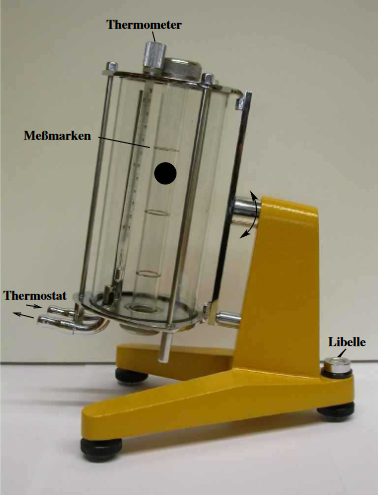
\includegraphics[width=0.8\textwidth]{assets/viskosimeter.png}
  \caption{Das Kugelfall-Viskosimeter nach Höppler \cite{V207}.}
  \label{fig:viskosimeter}
\end{figure}
\noindent Abbildung \ref{fig:viskosimeter} zeigt das für den Versuch verwendete Viskosimeter. Es besteht im wesentlichen aus einem Fallrohr, welches an jedem Ende mit einem Stopfen 
versehen ist und einem Wasserbad, welches an ein Thermostat angeschlossen wird, sodass die Temperatur innerhalb des Fallrohres variiert werden kann. Diese Apparatur ist an einem 
Gestell angebracht, welches es erlaubt die gesamte Apparatur zu drehen.
Für den Versuch werden zwei Glaskugeln mit unterschiedlichen Durchmessern genutzt. Zunächst werden die Durchmesser der beiden Kugeln mit einem Messschieber vermessen. Dann wird das 
Fallrohr des Viskosimeters mit destilliertem Wasser gefüllt und die kleinere Kugel wird in das Wasser hineingelassen. Es wird dabei darauf geachtet, dass keine Bläschen innerhalb des 
Fallrohres entstehen. Das Fallrohr wird mit den Stopfen verschlossen. Nun wird die Apparatur umgedreht, sodass die Kugel das Fallrohr hinabgleitet. Mit einer Stoppuhr wird die Zeit 
gemessen, die die Kugel benötigt um von der obersten Markierung bis zur untersten zu fallen. Die Länge der Fallstrecke beträgt dabei $l = \SI{10}{cm}$. Die Apparatur wird dann wieder 
umgedreht, sodass die Kugel wiederum durch das Rohr fällt und es wird wieder die Zeit gemessen, die die Kugel braucht um von der obersten Markierung zr untersten zu fallen. Dieser 
Vorgang wird wiederholt, bis insgesamt 20 Messwerte (10 Messwerte für jede Richtung) für die Fallzeit der Kugel aufgenommen wurden. Danach wird dieser Ablauf für die grße Kugel 
wiederholt, hierbei wird allerdings nur die Zeit gemessen, die die Kugel braucht um von der oberen Markierung zur mittleren zu fallen (Fallhöhe $l = \SI{5}{cm}$). Um die Temperaturabhängigkeit der dynamischen Viskosität zu bestimmen, wird die große Kugel verwendet. Während der erste Teil des Versuches bei Raumtemperatur stattfindet, 
wird nun das Thermostat genutzt um die Temperatur innerhalb des Viskosimeters zu erhöhen. Nachdem eine Temperatur am Thermostat eingestellt und das Wasserbad diese erreicht hat, 
wird etwa 2 Minuten gewartet, damit sich die Temperatur auch innerhalb des Fallrohres einstellen kann. Für jede Temperatur werden nun wie zuvor die Fallzeiten der Kugel von der 
obersten bis zur mittleren Markierung gemessen. Es werden 4 Fallzeiten gemessen (2 für jede Richtung), bevor die Temperatur weiter erhöht wird. Dieser Vorgang wird für 10 
verschiedene Temperaturen zwischen Raumtemperatur und $50^\circ \text{C}$ durchgeführt.